\documentclass[conference]{IEEEtran}
\IEEEoverridecommandlockouts
% The preceding line is only needed to identify funding in the first footnote. If that is unneeded, please comment it out.
\usepackage{cite}
\usepackage{amsmath,amssymb,amsfonts}
\usepackage{algorithmic}
\usepackage{graphicx}
\usepackage{textcomp}
\usepackage{xcolor}
\usepackage{url}
\usepackage[T1]{fontenc}
\usepackage[utf8]{inputenc}
\def\BibTeX{{\rm B\kern-.05em{\sc i\kern-.025em b}\kern-.08em
    T\kern-.1667em\lower.7ex\hbox{E}\kern-.125emX}}
\begin{document}

\title{Zvučni efekti na gitari\\
%{\footnotesize \textsuperscript{*}Note: Sub-titles are not captured in Xplore and
%should not be used}
%\thanks{Identify applicable funding agency here. If none, delete this.}
}

\author{\IEEEauthorblockN{Magdalena Halusek}
\IEEEauthorblockA{\textit{dept. name of organization (of Aff.)} \\
\textit{name of organization (of Aff.)}\\
City, Country \\
email address}\\
\IEEEauthorblockN{Ivana Šarić}
\IEEEauthorblockA{\textit{dept. name of organization (of Aff.)} \\
\textit{name of organization (of Aff.)}\\
City, Country \\
email address}
\and
\IEEEauthorblockN{Katarina Prgeša}
\IEEEauthorblockA{\textit{dept. name of organization (of Aff.)} \\
\textit{name of organization (of Aff.)}\\
City, Country \\
email address}\\
\IEEEauthorblockN{Ivana Žeger}
\IEEEauthorblockA{\textit{dept. name of organization (of Aff.)} \\
\textit{name of organization (of Aff.)}\\
City, Country \\
email address}
\and
\IEEEauthorblockN{Karla Salamun}
\IEEEauthorblockA{\textit{dept. name of organization (of Aff.)} \\
\textit{name of organization (of Aff.)}\\
City, Country \\
email address}
}

\maketitle

\renewcommand{\figurename}{Slika}

\begin{abstract}
sažetak??
\end{abstract}

\begin{IEEEkeywords}
component, formatting, style, styling, insert
\end{IEEEkeywords}

\section{Uvod}
Zvuk je mehanički val koji se prenosi određenim medijem. Ljudsko uho je osjetljivo na
frekvencije između otprilike 20 Hz i 20 000 Hz. Jedan je od mnogih oblika kontinuiranih;
analognih signala naše okoline. Ljudski interes za fenomen zvuka traje od najranije povijesti. Do
današnjice je razvijena čitava kultura i tehnologija koja omogućuje stvaranje, snimanje, obradbu
i prijenos zvuka. Pojam povezan sa zvukom koji obuhvaca i ispreplice znanost i umjetnost je glazba.
S ciljem što boljeg doživljaja glazbe, audio signali se obrađuju u kontinuiranoj i
diskretnoj domeni. Mikrofon pretvara zvučne valove u analogni električni sinusni signal. Taj je
signal određen jedinstvenom frekvencijom, brzinom, odstupanjima, itd. Obradba analognim
sklopovima podložna je pogreškama uzrokovanih šumom, preslušavanjem vodova,
temperaturnom ovisnošću, netočnostima nominalnih iznosa elemenata, itd. Da bi se kvalitetno
obradio, kontinuirani signal je potrebno digitalizirati. Digitalna obrada signala se provodi u
računalima. Ima brojne prednosti, poput neosjetljivosti na šum i starenje, laku prilagodbu na
nove zadatke, programabilnost.

Tema projekta je konstruiranje filtara za dodavanje efekata, digitalna obradba snimljenog zvuka
gitare primjenom istih te ispitivanje njihovog utjecaja na signal u vremenskoj i frekvencijskoj
domeni. Razvoj instrumenata i postupaka digitalne obradbe omogućio je eksperimentiranje
zvukom. Glazba se često razvijala upravo iz razloga što su pojedine slučajne greške u sviranju
instrumenata i obradbi snimaka zvuka postale utjecajni zvučni efekti. Zvučni efekti su pojam koji
obuhvaća hardver i softver odgovoran za manipulaciju zvukom. Moguće ih je dodati zvuku u
procesu nastajanja s ciljem da kasnije budu filtrirani ili preoblikovani \cite{b1}, ili
na kraju obrade, u produkcijskoj fazi. Ne postoji jedinstveno pravilo koje je potrebno slijediti pri
odabiru redoslijeda primjene efekata. No, promijenjeni redoslijed uzrokuje promjenu zvuka.
Potrebno je voditi računa o spomenutom obzirom na zvuk koji je poželjno stvoriti. Iako postoje
mnoge vrste i podjele, kao temeljna podjela digitalnih zvučnih efekata
može se navesti sljedeća:
\section{Introduction}
This document is a model and instructions for \LaTeX.
Please observe the conference page limits.

\section{Ease of Use}

\subsection{Maintaining the Integrity of the Specifications}

The IEEEtran class file is used to format your paper and style the text. All margins,
column widths, line spaces, and text fonts are prescribed; please do not
alter them. You may note peculiarities. For example, the head margin
measures proportionately more than is customary. This measurement
and others are deliberate, using specifications that anticipate your paper
as one part of the entire proceedings, and not as an independent document.
Please do not revise any of the current designations.

\section{Efekti temeljeni na kašnjenju}

\subsection{Jeka}

\section{Prepare Your Paper Before Styling}
Before you begin to format your paper, first write and save the content as a
separate text file. Complete all content and organizational editing before
formatting. Please note sections \ref{AA}--\ref{SCM} below for more information on
proofreading, spelling and grammar.

Keep your text and graphic files separate until after the text has been
formatted and styled. Do not number text heads---{\LaTeX} will do that
for you.

\subsection{Abbreviations and Acronyms}\label{AA}
Define abbreviations and acronyms the first time they are used in the text,
even after they have been defined in the abstract. Abbreviations such as
IEEE, SI, MKS, CGS, ac, dc, and rms do not have to be defined. Do not use
abbreviations in the title or heads unless they are unavoidable.

\subsection{Units}
\begin{itemize}
\item Use either SI (MKS) or CGS as primary units. (SI units are encouraged.) English units may be used as secondary units (in parentheses). An exception would be the use of English units as identifiers in trade, such as ``3.5-inch disk drive''.
\item Avoid combining SI and CGS units, such as current in amperes and magnetic field in oersteds. This often leads to confusion because equations do not balance dimensionally. If you must use mixed units, clearly state the units for each quantity that you use in an equation.
\item Do not mix complete spellings and abbreviations of units: ``Wb/m\textsuperscript{2}'' or ``webers per square meter'', not ``webers/m\textsuperscript{2}''. Spell out units when they appear in text: ``. . . a few henries'', not ``. . . a few H''.
\item Use a zero before decimal points: ``0.25'', not ``.25''. Use ``cm\textsuperscript{3}'', not ``cc''.)
\end{itemize}

\subsection{Equations}
Number equations consecutively. To make your
equations more compact, you may use the solidus (~/~), the exp function, or
appropriate exponents. Italicize Roman symbols for quantities and variables,
but not Greek symbols. Use a long dash rather than a hyphen for a minus
sign. Punctuate equations with commas or periods when they are part of a
sentence, as in:
\begin{equation}
a+b=\gamma\label{eq}
\end{equation}

Be sure that the
symbols in your equation have been defined before or immediately following
the equation. Use ``\eqref{eq}'', not ``Eq.~\eqref{eq}'' or ``equation \eqref{eq}'', except at
the beginning of a sentence: ``Equation \eqref{eq} is . . .''

\subsection{\LaTeX-Specific Advice}

Please use ``soft'' (e.g., \verb|\eqref{Eq}|) cross references instead
of ``hard'' references (e.g., \verb|(1)|). That will make it possible
to combine sections, add equations, or change the order of figures or
citations without having to go through the file line by line.

Please don't use the \verb|{eqnarray}| equation environment. Use
\verb|{align}| or \verb|{IEEEeqnarray}| instead. The \verb|{eqnarray}|
environment leaves unsightly spaces around relation symbols.

Please note that the \verb|{subequations}| environment in {\LaTeX}
will increment the main equation counter even when there are no
equation numbers displayed. If you forget that, you might write an
article in which the equation numbers skip from (17) to (20), causing
the copy editors to wonder if you've discovered a new method of
counting.

{\BibTeX} does not work by magic. It doesn't get the bibliographic
data from thin air but from .bib files. If you use {\BibTeX} to produce a
bibliography you must send the .bib files.

{\LaTeX} can't read your mind. If you assign the same label to a
subsubsection and a table, you might find that Table I has been cross
referenced as Table IV-B3.

{\LaTeX} does not have precognitive abilities. If you put a
\verb|\label| command before the command that updates the counter it's
supposed to be using, the label will pick up the last counter to be
cross referenced instead. In particular, a \verb|\label| command
should not go before the caption of a figure or a table.

Do not use \verb|\nonumber| inside the \verb|{array}| environment. It
will not stop equation numbers inside \verb|{array}| (there won't be
any anyway) and it might stop a wanted equation number in the
surrounding equation.

\subsection{Some Common Mistakes}\label{SCM}
\begin{itemize}
	\item{modulacijski efekti – \textit{Chorus}, \textit{Tremolo}, \textit{Flanger}, \textit{Phaser},}
	\item{vremenski efekti – \textit{Reverb}, kašnjenje, odjek,}
	\item{spektralni efekti – ekvilizacija, \textit{Panning},}
	\item{dinamički efekti – kompresija i distorzija.}
\end{itemize}

Tipični redoslijed efekata za gitaru \cite{b1} jest kompresija – distorzija – ekvilizacija – smanjenje šuma
– modulacija – kašnjenje – odjek.

Filtri po definiciji uklanjaju ili atenuiraju određene frekvencije iz spektra signala iznad
ili ispod neke granične frekvencije. Izjednačivači, pak, pojačavaju ili smanjuju određene frekvencijske
pojaseve, dok druge ne mijenjaju.


\section{Kompresija}

Kompresor djeluje na zvučni signal u cijelosti s ciljem kontrole zvuka i stvaranja \textit{sustain}
efekta. Kompresija je, zapravo, automatska kontrola glasnoće. Zadaća kompresora je smanjenje
dinamičkog raspona signala, tj. varijacije između najglasnijih i najtiših dijelova signala.
Dijelovi signala s velikim amplitudama, odnosno oni glasniji od nekog praga su atenuirani. Oni s
najmanjim amplitudama, tj. tiši od nekog praga su pojačani s namjerom postizanja uravnoteženijeg zvuka
bez distorzije. Kompresijom je omogućeno pojačanje signala bez potrebe za rezanjem (\textit{clippingom}).
Rezultat je dotjeraniji zvuk. Ipak, javlja se potreba za oprezom jer prekomjerna kompresija stvara
zašumljen i bezizražajan zvuk. Gubitak dijela dinamike postaje zamjetan pri slušanju.

Ovim projektom napravljen je kod za usporedbu originalnog i komprimiranog signala u vremenskoj i
frekvencijskoj domeni što je vidljivo na slici \ref{komp_vrijeme}.

\begin{figure}[h]
    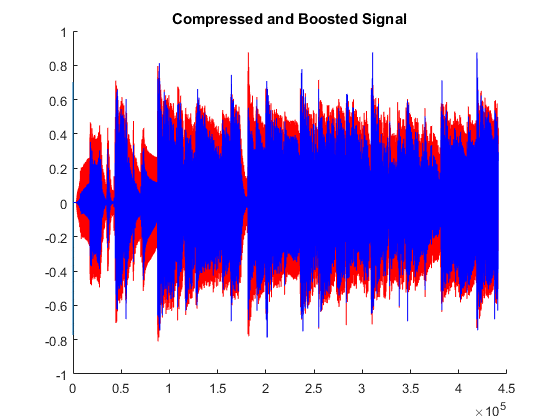
\includegraphics[scale=0.45]{slike/kompresija_vrijeme.png}
    \centering
    \caption{Originalni i komprimirani signal u vremenskoj domeni}							%dodati legend u matlabu
    \label{komp_vrijeme}
\end{figure}

Na slici \ref{komp_spektar} vidljiva je razlika u spektru. Budući da se događaju promjene u amplitudi u
vremenskoj domeni, to je u frekvencijskoj domeni vidljivo kao novonastala istosmjerna komponenta.

\begin{figure}[h]
    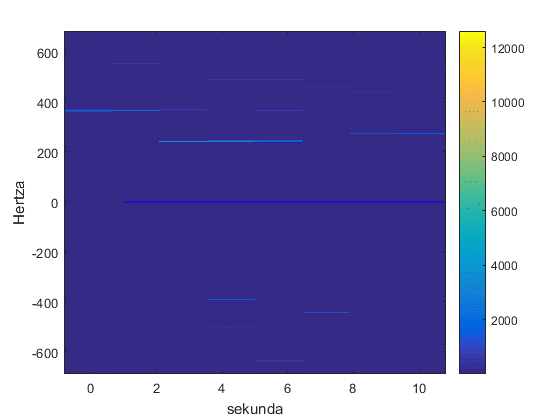
\includegraphics[scale=0.45]{slike/kompresija_spektar.png}
    \centering
    \caption{Spektrogram komprimiranog signala}							%zasto DC komponenta??
    \label{komp_spektar}
\end{figure}

\section{Zaključak}
Digitalna obradba signala sastavni je dio glazbene produkcije. Zvučni efekti, često nastali kao
posljedica slučajnih pogrešaka u sviranju i obradbi signala, glavni su faktori u manipulaciji zvukom.

Kompresija smanjuje dinamički raspon signala bez distorzije, bez potrebe za rezanjem
(\textit{clippingom}).

\begin{thebibliography}{00}
\bibitem{b1} Cardiff University, ``Digital Audio Effects'',
	\url{www.cs.cf.ac.uk/Dave/CM0268/PDF/10_CM0268_Audio_FX.pdf}
\end{thebibliography}

\end{document}
